% Created 2023-01-11 Ср 00:08
% Intended LaTeX compiler: pdflatex
\documentclass[PI, VKR]{HSEUniversity}
         \usepackage{array,tabularx,tabulary,booktabs,longtable,multirow}
         \Year{\the\year{}}
         \supervisor{к.т.н., доцент кафедры информационных технологий в бизнесе НИУ ВШЭ-Пермь}{А. В. Бузмаков}
                  \Abstract{В данной работе проведен анализ этичности разных компаний.

В первой главе находится описание используемых алгоримов.

Во второй главе представлено проектирование системы.

В третьей главе представлена реализация системы.

В четвертой главе представлено тестирование работы системы.

Количество страниц - N, количество иллюстраций - N, количетсво таблиц - N.}


\usepackage[utf8]{inputenc}
\usepackage[T1]{fontenc}
\usepackage{graphicx}
\usepackage{longtable}
\usepackage{wrapfig}
\usepackage{rotating}
\usepackage[normalem]{ulem}
\usepackage{amsmath}
\usepackage{amssymb}
\usepackage{capt-of}
\usepackage{hyperref}
\author{Соломатин Роман Игоревич}
\date{\today}
\title{Разработка сайта для автоматического сбора, анализа и визуализации информации по этичности компаний}
\hypersetup{
 pdfauthor={Соломатин Роман Игоревич},
 pdftitle={Разработка сайта для автоматического сбора, анализа и визуализации информации по этичности компаний},
 pdfkeywords={},
 pdfsubject={},
 pdfcreator={Emacs 28.2 (Org mode 9.6)},
 pdflang={Ru}}
\usepackage{biblatex}
\addbibresource{/home/samoed/Desktop/ESGanalysis/docs/library.bib}
\begin{document}

\maketitle

\chapter*{Введение}
\label{sec:org89a9856}
При работе с различными компаниями возникают проблемы их надежности, то как они ведут себя в спорных ситуациях, есть ли сервисы направленные на взаимодействие с клиентами.

В настоящее время существуют сервисы, которые могут оценить этичность компании на основании судебных дел, но не на отзывах о компании.

Объект исследования – деятельность компаний.

Предмет исследования – программные средства для оценки этичности деятельности компаний.

Цель работы – создание системы для оценки этичности компаний.

Исходя из поставленной цели, необходимо:

\begin{enumerate}
\item Провести анализ предметной области
\item Провести анализ системы
\item Реализовать систему
\item Провести тестирование системы
\end{enumerate}

Этап анализа должен:
\begin{enumerate}
\item Анализ предметной области
\item Анализ существующих алгоритмов
\end{enumerate}

Этап проектирования должен включать:
\begin{enumerate}
\item Проектирование серверной части
\item Проектирование модели для определения этичности
\item Проектирование клиентской части приложения
\end{enumerate}

Этап реализации должен включать:
\begin{enumerate}
\item Описание сбора данных
\item Реализации модели
\item Реализации серверной части
\item Реализации клиентской части
\end{enumerate}

Этап тестирования должен включать:
\begin{enumerate}
\item Тестирование модели
\item Тестирование серверной части
\item Тестирование клиентской части
\end{enumerate}
\chapter{Анализ предметной области}
\label{sec:orgabd4fa9}
\section{Постановка задачи}
\label{sec:orga7787f5}
В данный момент при выборе компаний приходится смотреть отзывы на различных сайтов и самому анализировать на сколько этична компания.
\section{BERT}
\label{sec:orgb326b46}
BERT \autocite{devlin2018bert} (Bidirectional Encoder Representations from Transformers) -- это нейросетевая языковая модель, которая относится к классу трансформеров. Она состоит из 12 «базовых блоков» (слоев), а на каждом слое 768 параметров.

На вход модели подается предложение или пара предложений. Затем разделяется на отдельные слова (токены). Потом в начало последовательности токенов вставляется специальный токен \texttt{[CLS]}, обозначающий начало предложения или начало последовательности предложений. Пары предложений группируются в одну последовательность и разделяются с помощью специального токена \texttt{[SEP]}, затем к каждому токену добавляется эмбеддинг, показывающий к какому предложению относится токен. Потом все токены превращаются в эмбеддинги \ref{fig:inputemebeddings} по механизму описаному в работе \autocite{NIPS2017_3f5ee243}.

\begin{figure}[h]
\centering
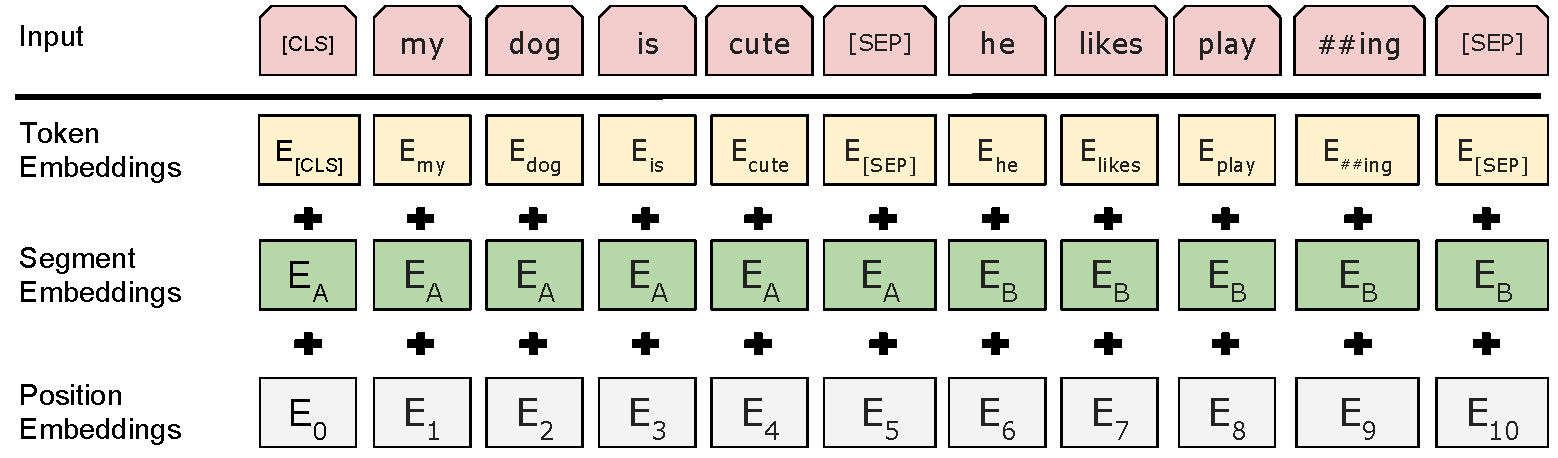
\includegraphics[width=.9\linewidth]{img/Input_Emebeddings.pdf}
\caption{\label{fig:inputemebeddings}Пример ввода текста в модель}
\end{figure}

При обучении модель выполняет на 2 задания:
\begin{enumerate}
\item Предсказание слова в предложении

Поскольку стандартные языковые модели либо смотрят текст слева направо или справа налево \ref{fig:BERT_comparisons}, как ELMo\autocite{elmo} и GPT\autocite{radford2019language}, они не подходят под некоторые типы заданий. Так как BERT двунаправленный, у каждого слова можно посмотреть его контекст, что позволит предсказать замаскированное слово.

\begin{figure}[h]
\centering
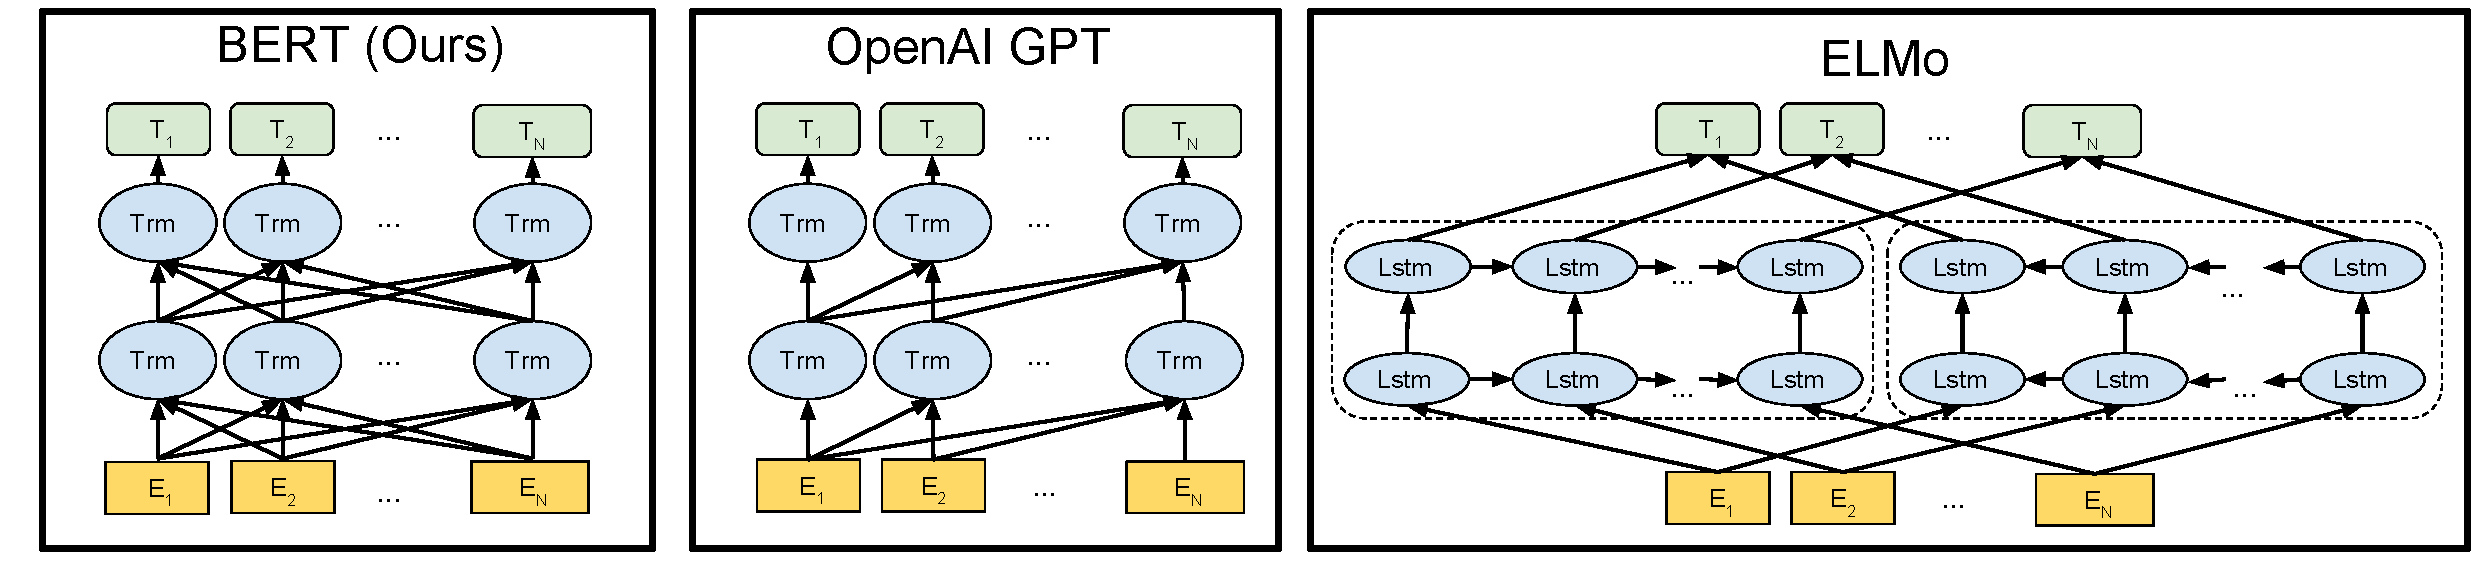
\includegraphics[width=.9\linewidth]{img/BERT_comparisons.pdf}
\caption{\label{fig:BERT_comparisons}Сравнение принципов работы BERT, ELMo, GPT}
\end{figure}

Это задание обучается следующим образом -- 15\% случайных слов заменяются в каждом предложении на специальный токен \texttt{[MASK]}, а затем предсказываются на основании контекста. Однако иногда слова заменяются не на специальны токена, в 10\% заменяются на случайный токен и еще в 10\% заменяются на случайное слово.

\item Предсказание следующего предложения

Для того чтобы обучить модель, которая понимает отношения предложений, она предсказывает, идут ли предложения друг за другом. Для этого с 50\% вероятностью выбирают предложения, которые находятся рядом и наоборот. Пример ввода пары предложений в модель \ref{fig:bert_pretrainin}.

\begin{figure}[hbp]
\centering
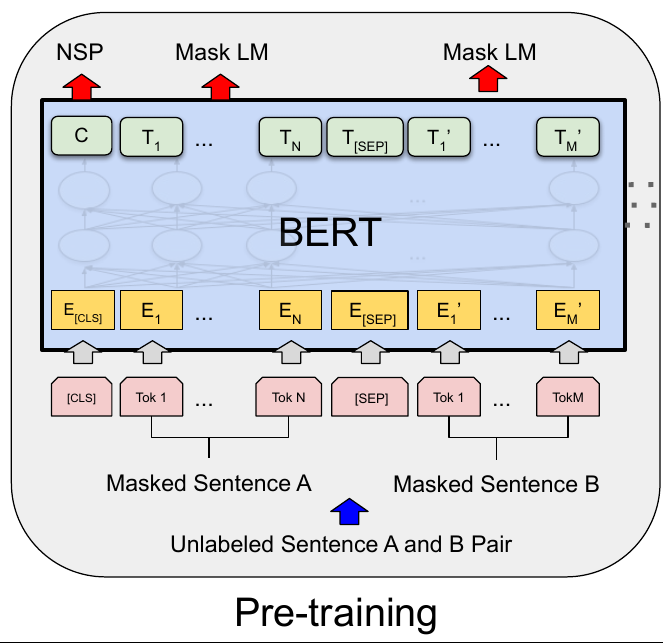
\includegraphics[width=0.6\textwidth]{img/bert_pretrainin.png}
\caption{\label{fig:bert_pretrainin}Схемам работы BERT}
\end{figure}
\end{enumerate}
\section{Sentense BERT}
\label{sec:orgc527cc8}
Sentense BERT \autocite{reimers-2019-sentence-bert} -- это модификация предобученных моделей BERT, которая использует 2 модели BERT, затем усреднят их выходы, а после с помощью функции ошибки выдаёт результат. Схема работы модели \ref{fig:sbert} \ref{fig:sbert}.
\begin{figure}[hbp]
\centering
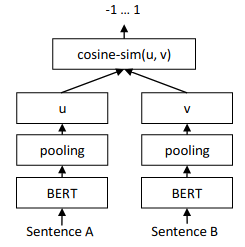
\includegraphics[width=0.6\textwidth]{img/sbert.png}
\caption{\label{fig:sbert}Схема работы SBERT}
\end{figure}
Основное преимущество данной модели над классическим BERT: эмбеддинги предложений можно сравнивать друг с другом независимо и не пересчитывать их пару каждый раз. Например, если для поиска похожих предложений из 10000 для обычного BERT потребуется 50 миллионов вычислений различных пар предложений, и это займёт 50 часов, то Sentense BERT рассчитает эмбеддинг каждого предложения отдельно и потом их сравнит, и это займёт примерно 5 секунд.
\chapter{Проектирование системы}
\label{sec:orga64e340}
\section{Проектирование базы данных}
\label{sec:orgd1afeb9}

\section{Проектирование архитектуры системы}
\label{sec:org002b2c7}
\begin{center}
\includegraphics[width=.9\linewidth]{img/mermaid/test.png}
\end{center}


\begin{center}
\includegraphics[width=.9\linewidth]{img/plantuml/tryout.png}
\end{center}

\subsection{Проектирование серверной части}
\label{sec:org3af2cea}
\subsection{Проектирование клиентской части}
\label{sec:org5f7deb1}

\chapter{Реализация системы}
\label{sec:org958a9ce}
\section{Реализация серверной части}
\label{sec:org2394a21}
\subsection{Реализация API}
\label{sec:orgf7c6129}
\subsection{Реализация парсера banki.ru}
\label{sec:orgc9a837a}
\subsection{Реализация парсера sravni.ru}
\label{sec:orgb920ead}
\subsection{Реализация модуля обработки текста}
\label{sec:orgc09b9a9}
\section{Реализация клиентской части}
\label{sec:org30f9240}
\chapter{Тестирование системы}
\label{sec:org84f65b2}
\chapter*{Заключение}
\label{sec:org508436a}
\nocite{*}
\putbibliography
\appendix
\end{document}
